\documentclass[11pt]{article}

\usepackage{tocloft}

\setcounter{tocdepth}{3}% to get subsubsections in toc

\usepackage{geometry}                % See geometry.pdf to learn the layout options. There are lots.
\geometry{a4paper}
\usepackage{graphicx}
\usepackage{amssymb}
\usepackage{epstopdf}

\setlength{\parskip}{0.25\baselineskip} % Espacio entre párrafos
\setlength{\parindent}{15pt} % Sangría en la primera línea de cada párrafo

\DeclareGraphicsRule{.tif}{png}{.png}{`convert #1 `dirname #1`/`basename #1 .tif`.png}

\usepackage[natbibapa]{apacite} % Cargar primero
\usepackage[spanish]{babel} % Si todavía no está cargado
\addto\captionsspanish{%
  \renewcommand{\figureautorefname}{Figura}%
  \renewcommand{\tableautorefname}{Tabla}%
  \renewcommand{\sectionautorefname}{Sección}%
  \renewcommand{\subsectionautorefname}{Subsección}%
  \renewcommand{\subsubsectionautorefname}{Subsubsección}%
  \renewcommand{\BRetrievedFrom}{Recuperado de }%
}

\usepackage{titlesec}
\titlelabel{\thetitle\quad}  % Esto elimina el punto

\usepackage{hyperref} % Para autoref

\titleformat{\section}
  {\normalfont\Large\bfseries}
  {\thesection}{1em}{}

\titleformat{\subsection}
  {\normalfont\large\bfseries}
  {\thesubsection}{1em}{}

\titleformat{\subsubsection}
  {\normalfont\normalsize\bfseries}
  {\thesubsubsection}{1em}{}

\renewcommand{\refname}{}

\newcommand{\titulolargo}{Generación de itinerarios de viaje a partir del procesamiento de correos electrónicos de reservas}

\usepackage{placeins}

\title{\titulolargo}
\author{Alumno: Meola, Franco Román (Leg. Nº 52163)}
%\date{}                                           % Activate to display a given date or no date

\newcommand{\titulocorto}{TFI - ECD 2024B - Ing. Franco Román Meola}
\makeatletter

\def\@evenhead{\normalfont\hfil \titulocorto \hfil}
\def\@oddhead{\normalfont\hfil \titulocorto \hfil}
\def\@evenfoot{\hfil \raisebox{-20pt}{\thepage} \hfil}
\def\@oddfoot{\hfil \raisebox{-20pt}{\thepage} \hfil}
\makeatother

\AtBeginDocument{%
  \renewcommand{\BOthers}[1]{et al}%
}

\begin{document}

\begin{titlepage}
\centering
\vspace*{1cm}


\includegraphics[width=0.25\textwidth]{images/itba-logo.png}\\[0.5cm]

\textsc{Instituto Tecnológico de Buenos Aires}\\[2cm]

\Huge \textbf{\titulolargo}\\[2cm]

\Large Alumno: Meola, Franco Román (Leg. Nº 52163)\\[0.5cm]

\Large Profesores: Mon, Alicia Laura y Kuna, Horacio Daniel\\[0.5cm]

\Large Taller: Trabajo Final Integrador - Especialización en Ciencia de Datos\\[0.5cm]

\Large Tutora: Dra. Leticia Irene Gómez\\[2.5cm]

\Large Buenos Aires\\[0.5cm]
\Large Primer Cuatrimestre, 2025

\vfill

\end{titlepage}

\pagebreak

\tableofcontents % Indice
\thispagestyle{empty}

\pagebreak

\FloatBarrier
\section{Introducción}

En la actualidad la organización eficiente de la información vinculada a viajes se ha convertido en un desafío. Es común que para el armado de un viaje se recurran a varios proveedores distintos de servicios turísticos. Si se realiza una compra en el sitio web de la aerolínea (por ejemplo a través de Lufthansa) el cliente recibirá en su bandeja de entrada un correo electrónico con todos los datos de su reserva. Cuando luego se realice la reserva del hotel es probable que utilice un sitio web diferente (por ejemplo a través de Booking.com) y obtenga otro correo electrónico distinto con los datos de la estadía. También es posible que durante el viaje se programen vuelos locales o regionales que involucren otras aerolíneas distintas (por ejemplo Ryanair).

Para poder consultar información importante como el aeropuerto de origen del vuelo o el horario de check-out del hotel el usuario tiene que estar consultando correos electrónicos distintos. Aunque estas empresas proveedoras de servicios turísticos ofrecen también aplicaciones móviles, tampoco se consigue una vista integral ya que el usuario deberá descargar y consultar una aplicación para el vuelo de ida, otra aplicación diferente para el hotel y quizás otra aplicación distinta para algún vuelo regional.

Además, al momento de darle un vistazo a los correos electrónicos o las distintas aplicaciones, cada una presenta una interfaz distinta donde es probable que el aeropuerto de origen del vuelo en el mail de una aerolínea esté arriba a la izquierda mientras que en otra aparezca en el centro. Estructuras distintas para diferentes proveedores obligan a que, para lograr una vista integral de la información, el usuario termine copiando esa información en otra parte, corriendo el riesgo de cometer un error o de contar con información desactualizada. 

Es por eso que es importante contar con una aplicación capaz de extraer información relevante de correos electrónicos de reservas independientemente de la estructura o el remitente del correo para luego proceder a la creación de un itinerario del viaje integral. 

El presente proyecto se centrará en la extracción de información relevante contenida exclusivamente en correos electrónicos de reservas de tickets aéreos y de estadías de hotel. Si bien se excluyen otros tipos de reserva (como alquileres de vehículos, pasajes de tren o reservas de restaurantes) se buscará diseñar una solución extensible en caso de que se desee ampliar el dominio en el futuro.

Asimismo, el alcance del trabajo abarca el desarrollo de un prototipo funcional que permita validar las técnicas aplicadas de extracción de información utilizando una solución web simple que simule ser la vista del usuario de la aplicación de gestión de itinerarios. No se contemplarán requisitos funcionales y no funcionales propios de una aplicación real orientada a un gran volumen de usuarios, tales como usabilidad, alta disponibilidad y seguridad.
 
\FloatBarrier
\section{Definición del problema}

La diversidad de sitios web para realizar la compra de vuelos y estadías en hoteles involucrados en el armado de un viaje produce correos electrónicos de confirmación con distintas estructuras provenientes de múltiples fuentes. El usuario, al momento de querer consultar el itinerario de un viaje, debe consultar cada uno de estos mails individualmente o interactuar con las respectivas aplicaciones de cada proveedor, dificultando una vista integral del itinerario completo.

\FloatBarrier
\section{Estado de la cuestión}

Se realizó un relevamiento de la literatura existente que cubre el procesamiento de correos electrónicos tanto de reservas de tickets aéreos como de estadías de hotel. Las estrategias propuestas abarcan desde métodos clásicos como el reconocimiento de entidades y clasificación basada en características estructurales del contenido de los correos hasta enfoques que utilizan técnicas de \textit{machine-learning} y generación automática de reglas de extracción.

Por un lado, trabajos como el de \cite{Kaushik2017} exploran el uso de técnicas de reconocimiento de entidades (\textit{Named Entity Recognition}) basadas en \textit{Hidden Markov Models} (HMM). De esta forma se busca rotular y extraer entidades relevantes incluso en escenarios con poca información contextual. Además proponen un conjunto de características específicas del dominio de reservas de tickets aéreos para enriquecer las predicciones. Cabe destacar que todos los autores de este artículo son parte de la división IT de Amadeus, una empresa líder en el ámbito de soluciones tecnológicas para viajes.

El abordaje de este problema a gran escala ha sido tratado por investigaciones como la de \cite{Sheng2018} cuyos autores son empleados de Google. Crearon un sistema para extraer información de correos electrónicos en un entorno como Gmail que atiende a más de mil millones de usuarios a diario. Su enfoque hace hincapié en tres principios: escalabilidad, privacidad y adaptabilidad. La solución combina un conjunto de clasificadores especializados cuyos resultados son integrados mediante un sistema de reglas ligeras, aplicado a las reservas de hotel.

Otra solución a gran escala se detalla en el artículo de \cite{DiCastro2018} donde investigadores de Yahoo! Research abordan el problema con la generación automática de reglas de extracción a partir del \textit{clustering} o agrupamiento de los mensajes según su estructura. Esta propuesta también se enfoca en el dominio de las reservas de tickets aéreos.

Desde Microsoft Research, \cite{Iyer2019} introduce el enfoque \textit{Heterogeneous Data Extraction Framework} (HDEF), donde combina un modelo de aprendizaje automático (CRF) para obtener un etiquetado inicial con un algoritmo de síntesis que genera programas de extracción interpretables. Dichos programas son refinados en un proceso iterativo hasta alcanzar la calidad deseada. Este enfoque ha sido aplicado al dominio de reservas de tickets aéreos.

Por último, el trabajo de \cite{Kocayusufoglu2019}, también con la mayoría de autores trabajando en Google, se centra en el \textit{rich formatting} utilizado en los correos electrónicos generados por sistemas B2C, donde existe información valiosa que puede ser usada para aprender mejores representaciones. A diferencia de los artículos anteriormente mencionados (donde en una etapa de preprocesamiento se descarta el código HTML del correo electrónico para procesar únicamente texto plano) en esta propuesta se plantea aprender representaciones combinadas que integren tanto la estructura HTML como el contenido textual. Esta representación es utilizada para entrenar un clasificador orientado al dominio de reservas de hotel.

\subsection{Aplicaciones}

Se realizó además un relevamiento de soluciones existentes en la actualidad que atiendan el problema planteado. Se encontraron aplicaciones destinadas al usuario que realiza las reservas como así también soluciones B2B. En cuanto a las aplicaciones comerciales podemos mencionar TripIt, Kayak Trips y Tripsy. En el ámbito del software libre existe KDE Itinerary. Respecto a las soluciones B2B mencionaremos a la API de Amadeus.

A continuación desarrollaremos una solución comercial gratuita (TripIt), una solución de software libre (KDE Itinerary) y una solución B2B (Amadeus).

\FloatBarrier
\subsubsection{TripIt}

Existe en la actualidad una solución gratuita llamada \cite{tripit-home} que atiende el problema planteado donde un usuario puede reenviar correos electrónicos a una casilla particular de forma que la aplicación extrae información relevante de distintos tipos de reservas (como vuelos, hoteles, alquiler de vehículos, restaurantes, boletos de tren, entre otras). 

El usuario debe primero crear un usuario desde la web o desde la aplicación móvil, y luego puede reenviar sus correos electrónicos a la casilla plans@tripit.com. Cuando desde TripIt reciben un nuevo correo se procesa su contenido y se identifica el remitente (que debe coincidir con el usuario registrado en la aplicación) para luego agregar a un itinerario la información extraída, como se puede apreciar en la \autoref{fig:tripit}. El usuario puede descargar la versión móvil desde las tiendas de aplicaciones de iOS y Android o utilizar la versión web.

\begin{figure}[htbp]
    \centering
    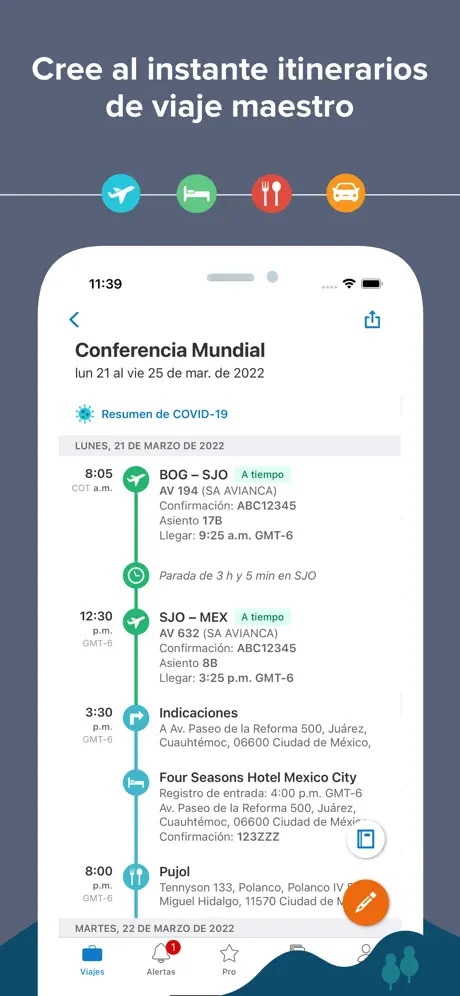
\includegraphics[width=0.20\textwidth]{images/tripit1.png}
    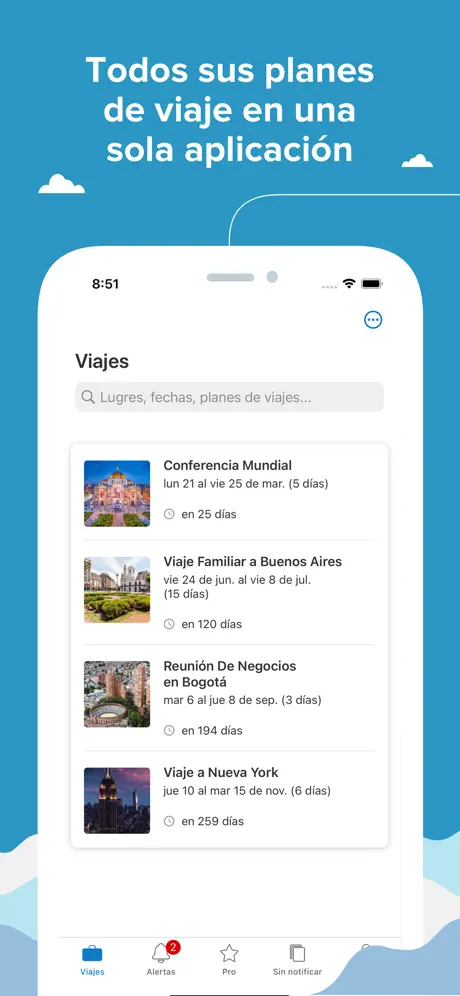
\includegraphics[width=0.20\textwidth]{images/tripit2.png}
    \caption{Capturas de pantalla de la aplicación TripIt}
    \label{fig:tripit}
\end{figure}

La aplicación no solo muestra una vista de itinerario integrada en función de los distintos correos electrónicos que se hayan reenviado sino que también permite agregar datos de eventos manualmente. También ofrece funcionalidad para obtener direcciones a puntos de interés (como el aeropuerto o la estación de tren) y en el caso de medios de transporte puede incluir alertas de cambio y retrasos.
 
Dado que es una solución comercial no se da a conocer cuáles son las técnicas que utiliza para procesar los correos electrónicos pero consultando en la documentación oficial se puede apreciar una lista de \textit{vendors} o proveedores de servicios de viaje que soporta la aplicación. Se mencionan cientos de proveedores distintos en correos electrónicos escritos en inglés, español, francés, alemán y japonés \cite{tripit-supported-sites}. Esta lista puede darnos un indicio de que la aplicación ha dedicado recursos para poder procesar cada uno de los correos electrónicos de los proveedores de servicios de viajes indicando que es probable que utilice una serie de plantillas predefinidas y un conjunto de reglas que se crean especialmente para cada proveedor.  

Un punto negativo a destacar sobre esta aplicación es la privacidad, es necesario reenviar a la aplicación correos electrónicos que contienen datos sensibles de los usuarios que son parte de la confirmación. Por ejemplo para una reserva de un ticket de vuelo en el mail aparecerán el nombre completo del usuario, número de pasaporte, nacionalidad, entre otros. 

\FloatBarrier
\subsubsection{KDE Itinerary}

En el ámbito del software libre se encuentra la aplicación \cite{kde-itinerary-home} que consiste en una solución enfocada en la privacidad del usuario. Utiliza una biblioteca KItinerary, también \textit{open-source}, que provee un motor de extracción de datos de correos electrónicos de viajes sin enviarlos a un servidor remoto. Al igual que TripIt, esta aplicación admite reservas de distinto tipo y ofrece actualizaciones en tiempo real para ciertos tipos de reserva. El usuario puede descargar la versión móvil (Ver \autoref{fig:kdeitinerary}) desde la tienda de aplicaciones de Android.

Luego de consultar el código fuente disponible en el repositorio oficial de \cite{k-itinerary-repo} se pueden apreciar actualizaciones frecuentes de la misma donde se indican cambios para soportar nuevos proveedores de servicios como así también para mantenerse al día con las actualizaciones de las estructuras de los correos electrónicos de proveedores ya soportados. En cuanto a la implementación se emplea una combinación de técnicas que incluyen detección de palabras clave, utilización de expresiones regulares para formatos comunes de fecha y hora, y ciertas heurísticas basadas en el contenido HTML del correo.

\begin{figure}[htbp]
    \centering
    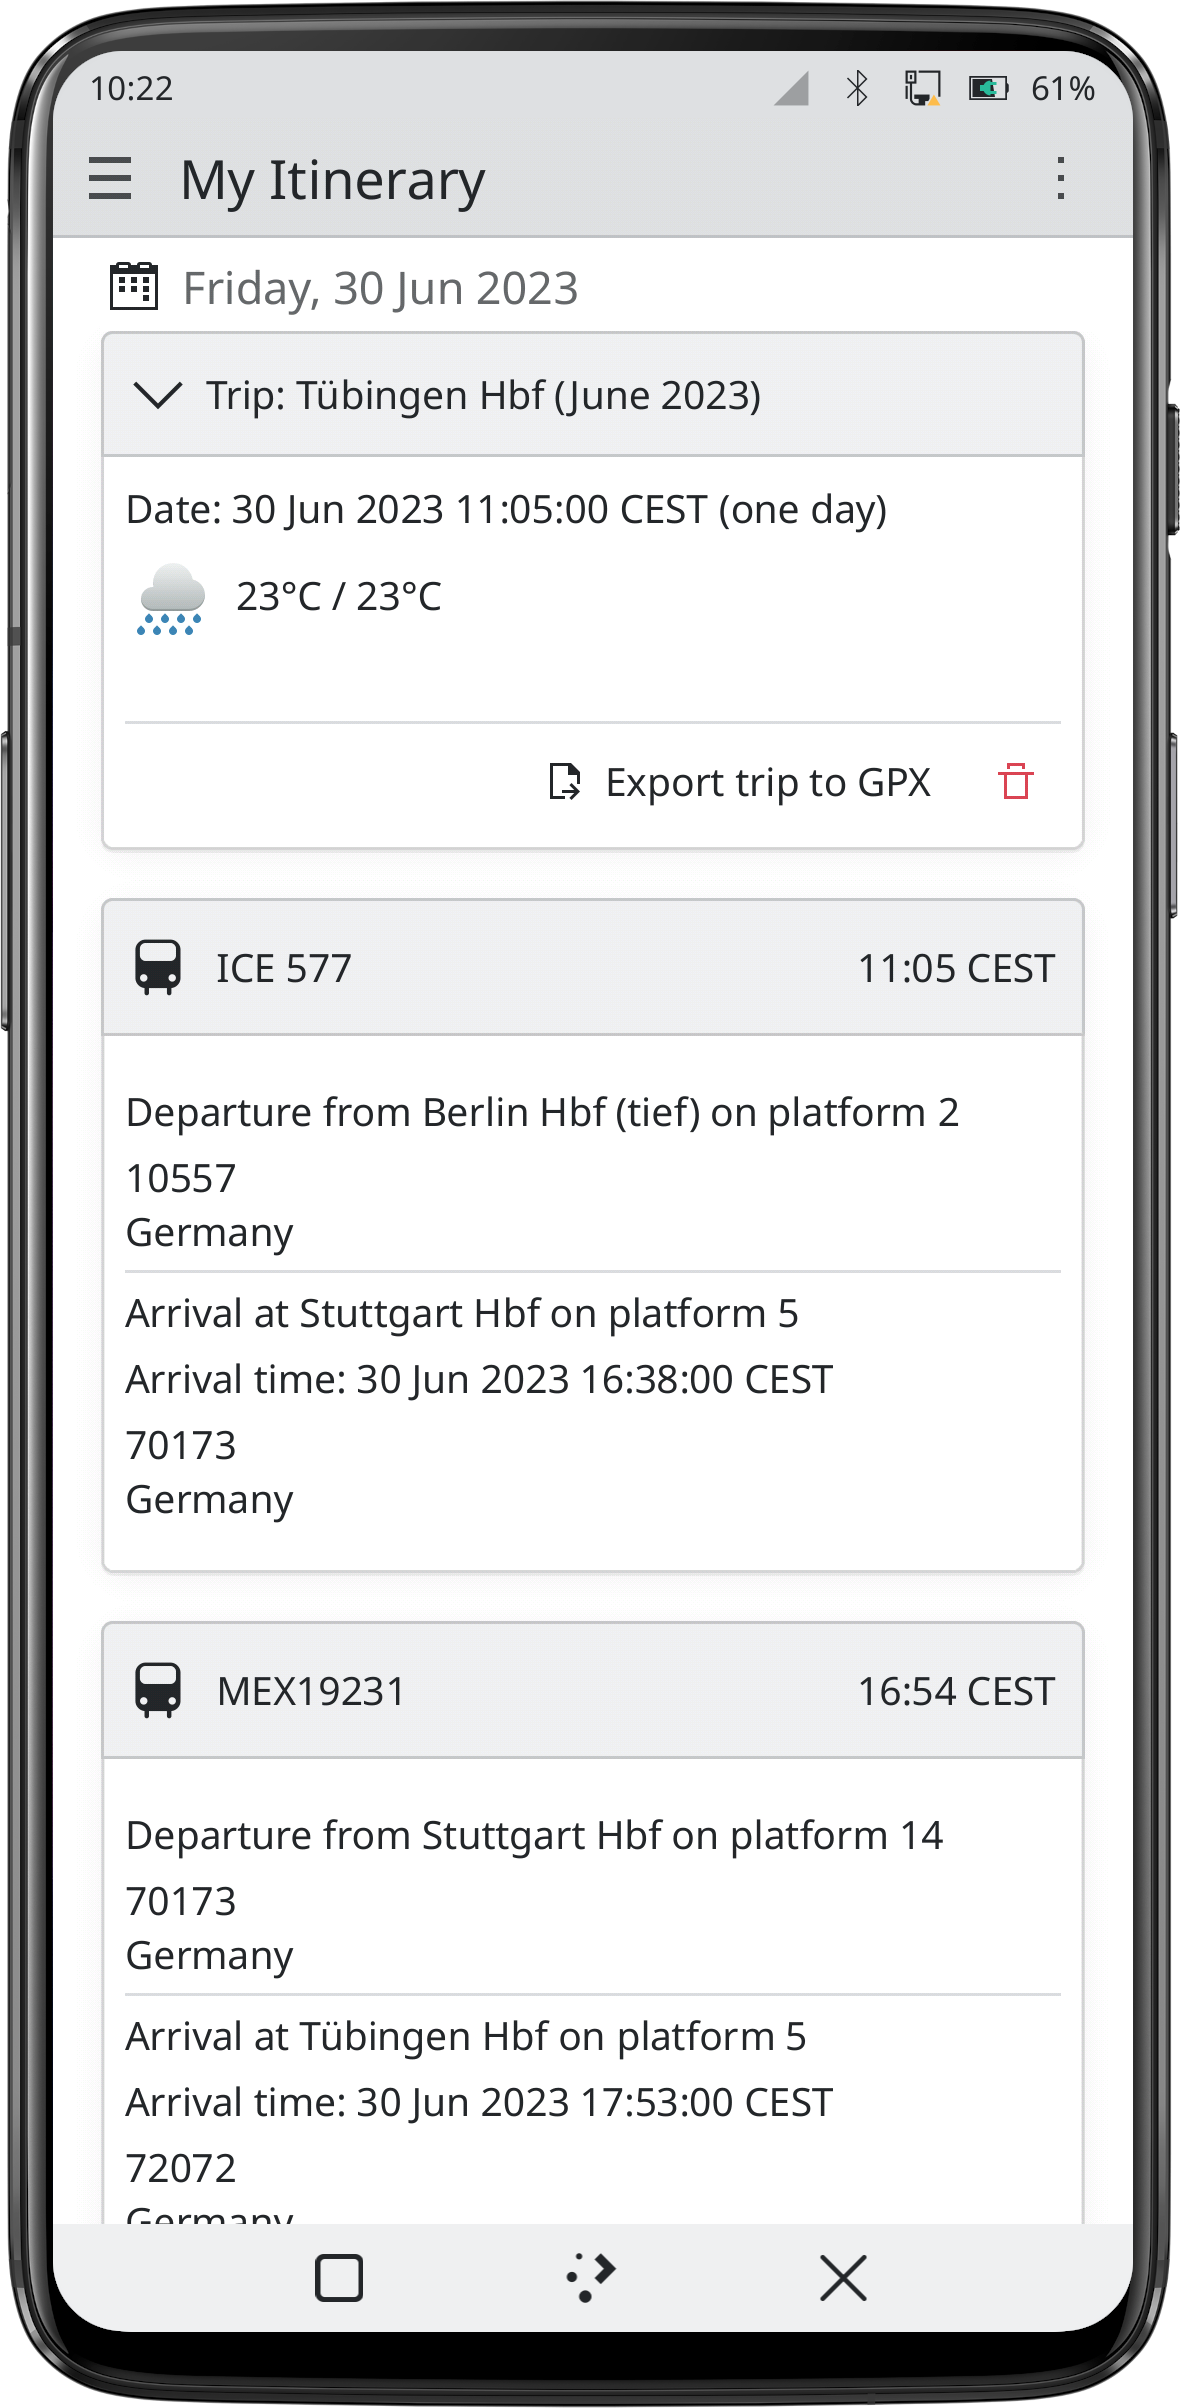
\includegraphics[width=0.20\textwidth]{images/kde1.png}
    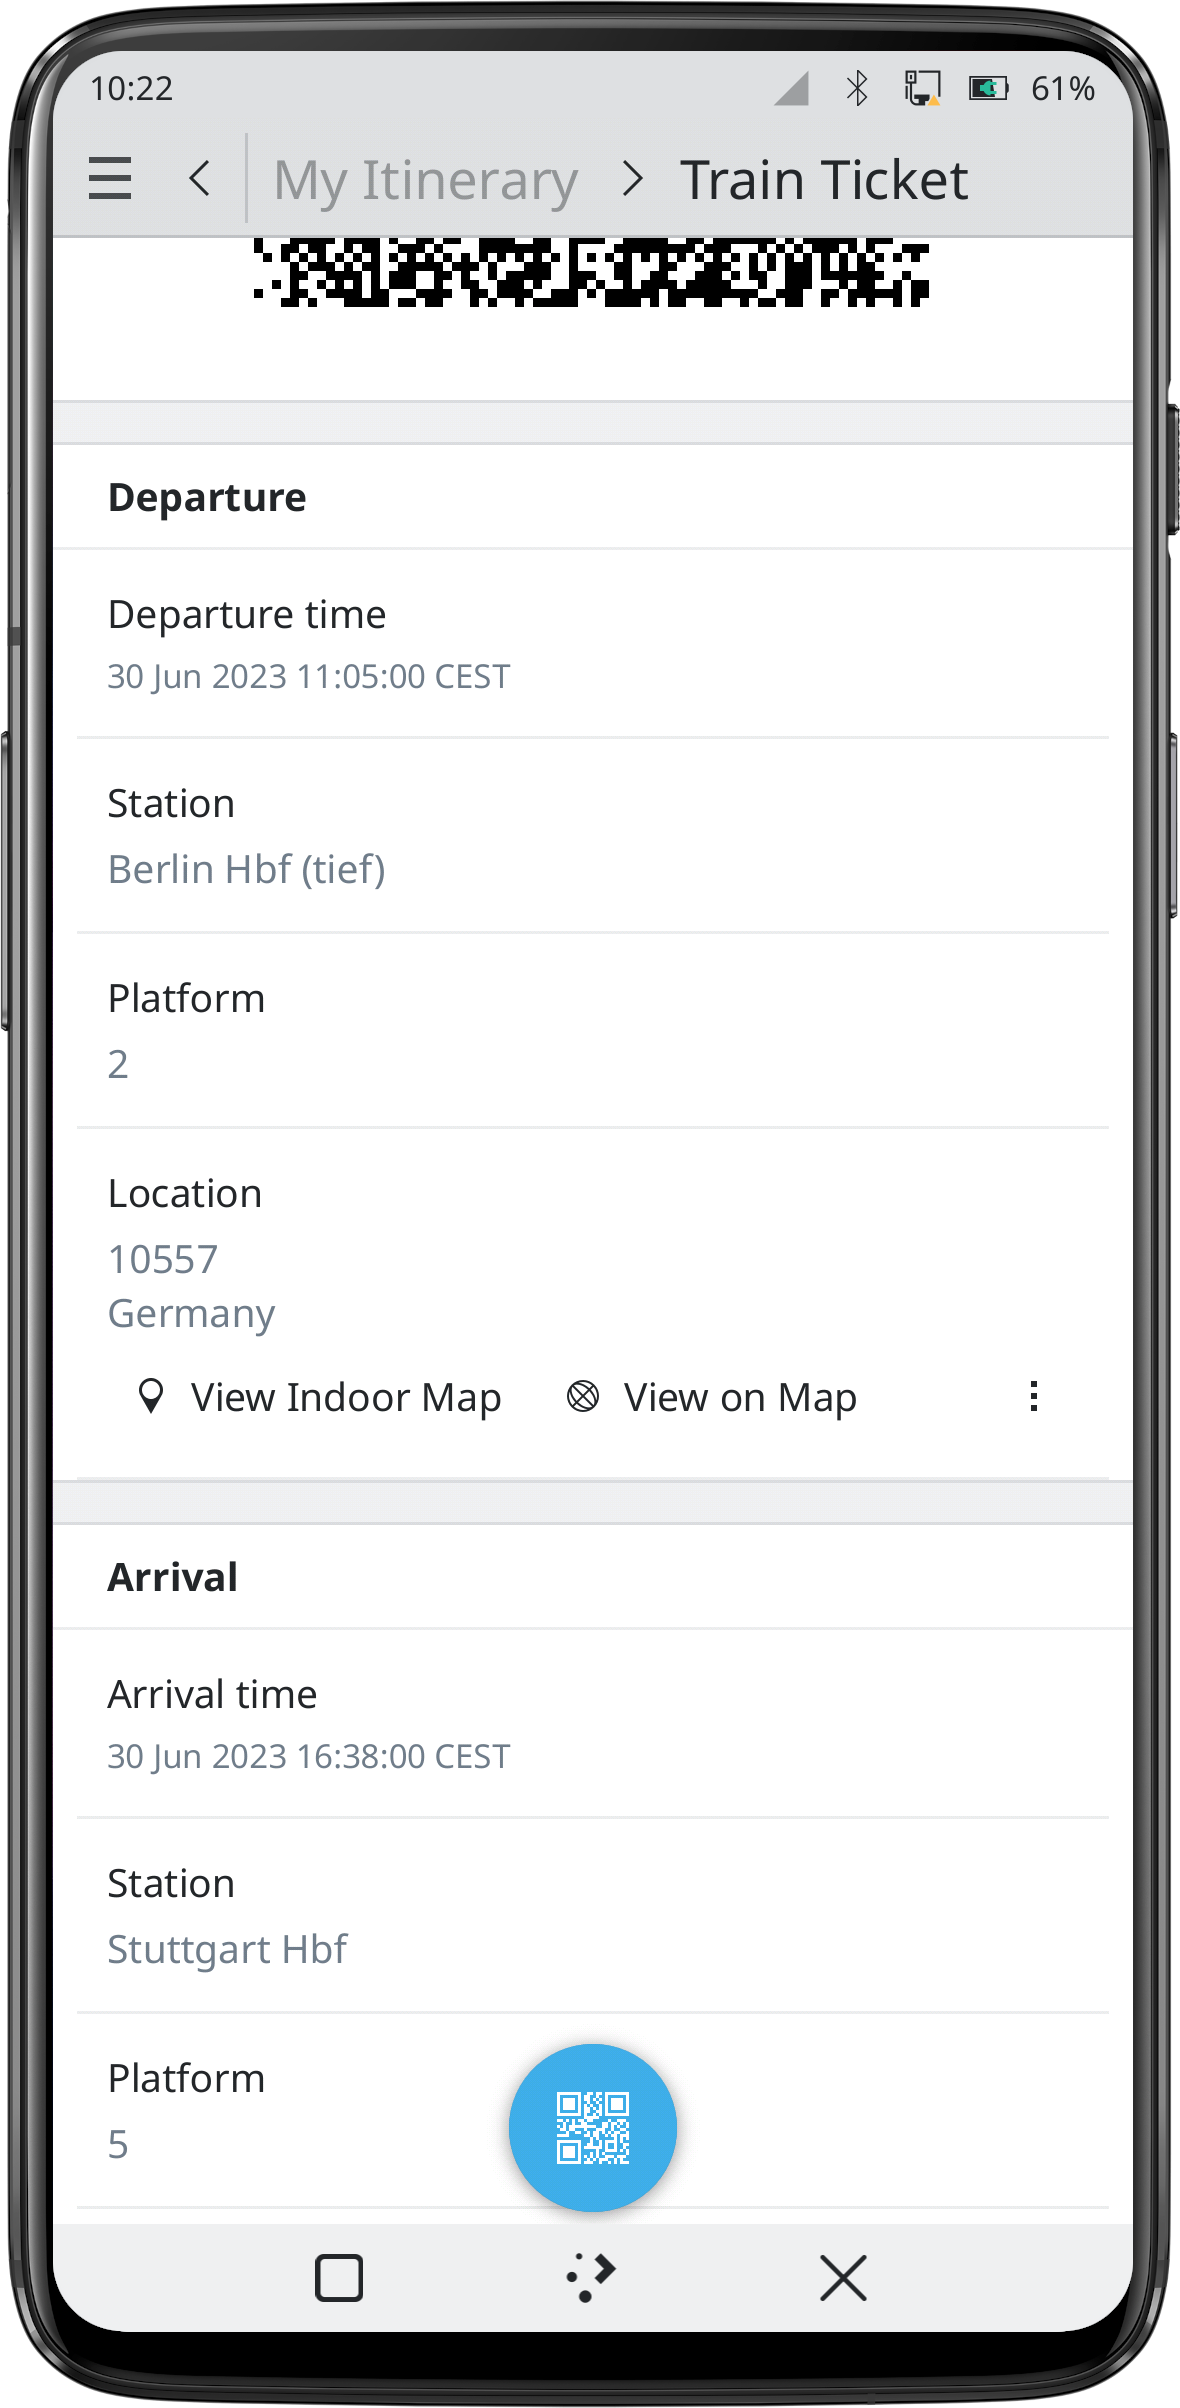
\includegraphics[width=0.20\textwidth]{images/kde2.png}
    \caption{Capturas de pantalla de la aplicación KDE Itinerary}
    \label{fig:kdeitinerary}
\end{figure}

\FloatBarrier
\subsubsection{Amadeus Self-Service APIs: Trip Parser}

Por último mencionamos la función de \cite{amadeus-trip-parser} perteneciente al servicio Self-Service APIs de Amadeus. Amadeus IT Group es una empresa líder en el ámbito del turismo que provee soluciones tecnológicas que abarcan los sistemas de reservas que utilizan aerolíneas, aeropuertos, proveedores de hospedaje y agencias de viajes entre otros. Amadeus ofrece un conjunto de APIs para permitir la integración de sistemas de terceros tanto para realizar y administrar reservas como así también ofrecer recomendaciones para futuras reservas. 

El servicio Trip Parser que ofrece Amadeus consiste en un método que recibe uno o varios correos electrónicos de reservas (codificados en el formato Base64) y extrae información de todos ellos agregándola en un único archivo JSON que contendrá toda la información del itinerario correspondiente. Esta solución paga para desarrolladores soporta contenido en HTML, EML y PDF de más de 300 proveedores distintos en 27 lenguajes y puede ser utilizada por cualquier aplicación web o móvil que quiera atender el problema planteado.

Cabe destacar que la API 
%(Ver \autoref{fig:amadeus}) 
ha sido deprecada por Amadeus por lo que es probable que deje de funcionar en un futuro.

%\begin{figure}[htbp]
%    \centering
%    \includegraphics[width=0.75\textwidth]{images/amadeus1.png}
%    \caption{Sitio web de Trip Parser del portal de desarrolladores de Amadeus}
%    \label{fig:amadeus}
%\end{figure}

\FloatBarrier
\section{Hipótesis}

Es posible generar una vista integral de la información de reservas de viaje a partir de la extracción de datos relevantes presentes en los mails de confirmación, independientemente del proveedor de servicio y de la estructura de mail utilizada.  

\subsection{Variables}

A continuación se detalla el primer conjunto de variables a ser adoptadas para su tratamiento, clasificadas según su tipo (independiente, dependiente o contextual):

\begin{itemize}
\item \textbf{Datos relevantes (variable dependiente):} Para reservas de vuelos se debe extraer el nombre del pasajero, el código de reserva, la fecha y hora de salida y llegada, el aeropuerto de salida y llegada y datos del vuelo como el código y la aerolínea. En el caso de reservas de hoteles se debe extraer el nombre del hotel, la dirección, la fecha y hora de checkin y checkout. 
\item \textbf{Mails de confirmación (variable independiente)}: El contenido del mail de confirmación que contiene todos los datos relevantes en distintas formas de presentación.
\item \textbf{Reservas de viaje (variable dependiente)}: Reservas de vuelos y reservas de hoteles.
\item \textbf{Proveedor del Servicio (variable contextual)}: El emisor del mail de confirmación, un sitio web que realiza la reserva (por ejemplo Booking, sitios web de las aerolíneas, etc).
\item \textbf{Estructura del mail (variable contextual)}: Como se organiza el texto del mail a analizar.
\end{itemize}

\FloatBarrier
\section{Objetivos}

A continuación se presentan el objetivo general como así los objetivos específicos a los que apunta el presente proyecto.

\subsection{Objetivo General}

Implementar un modelo que permita identificar, clasificar y extraer automáticamente información relevante contenida en correos electrónicos de confirmación de reservas de vuelos y hoteles, independientemente del proveedor del servicio y de la estructura del correo.

\subsection{Objetivos Específicos}

\begin{itemize}
\item Investigar estrategias de procesamiento de lenguaje natural adecuadas para abordar textos con estructuras heterogéneas en correos electrónicos.
\item Diseñar y entrenar modelos de clasificación capaces de distinguir entre correos de reservas de vuelos y de hoteles sin depender del proveedor.
\item Implementar y comparar modelos de extracción de entidades que permitan recuperar con precisión los campos clave de cada tipo de reserva.
\item Analizar el impacto del preprocesamiento textual en el rendimiento de los modelos de clasificación y extracción.
\item Definir y aplicar métricas de evaluación que permitan medir la efectividad del sistema propuesto en tareas de clasificación y extracción de datos.
\end{itemize}

\FloatBarrier
\section{Metodología}

Para estructurar las fases de desarrollo del proyecto y la gestión de los objetivos específicos se aplicará una combinación de \textit{Scrum} con \textit{Crisp-DM}. Se detallan a continuación ambas metodologías, junto con las técnicas y herramientas a utilizar:

\subsection{Metodología Scrum + Crisp-DM}

\subsubsection{Scrum}

\textit{Scrum} es un marco de trabajo que posibilita un proceso ágil y liviano para administrar y controlar el desarrollo de \textit{software}. Es iterativo e incremental y cada iteración o \textit{sprint} concluye con una pieza de \textit{software} ejecutable que incorpora nueva funcionalidad.

Se deben aplicar ciertas modificaciones ya que el equipo de trabajo estará conformado por un único integrante (también conocido como \textit{Single Scrum}), destacando que el autor del proyecto combinará los roles de Desarrollador, \textit{Product Owner} y \textit{Scrum Master}.   

En principio se planean seis \textit{sprints} con una duración de dos semanas cada una, de forma que la totalidad del proyecto contempla una duración aproximada de tres meses. Una vez definidas las historias de usuario se deberá proceder a dividirlas en tareas más pequeñas que terminarán formando parte del \textit{backlog} del proyecto.

Al finalizar cada \textit{sprint} se compartirá el avance hasta el momento con el/la tutor/a del proyecto para obtener la retroalimentación correspondiente.

Si bien su aplicación abarca la totalidad de las tareas del proyecto, se destaca para las potenciales tareas del desarrollo de \textit{software} que serán necesarias en este proyecto como la implementación del \textit{endpoint} que, a partir del contenido de un correo electrónico, extraiga la información relevante y también la implementación de una interfaz web simple que muestre el itinerario agregado de un usuario.

\subsubsection{Crisp-DM}

\textit{Crisp-DM} es una metodología para el desarrollo de proyectos de \textit{data mining} (DM) independiente de las herramientas de \textit{software}.

Esta metodología estructura el trabajo en seis fases: Comprensión del negocio, Análisis de los datos, Preparación de los Datos, Modelado, Evaluación y Despliegue.

Su aplicación permitirá en este proyecto guiar la potencial creación de modelos de clasificación de los correos electrónicos, la implementación de técnicas de extracción de información y la evaluación de los resultados obtenidos.  

\subsection{Técnicas}

En cuanto a las técnicas, en primer lugar se utilizarán tokenización y normalización, provenientes del área del procesamiento de lenguaje natural (NLP). Para la clasificación de los correos electrónicos según el tipo de reserva que contengan se utilizarán modelos de aprendizaje supervisado. También se utilizará Named Entity Recognition para poder extraer la información relevante de cada mail de reserva, con la ayuda de expresiones regulares para aquellos casos que respeten patrones predecibles.

\subsection{Herramientas}

Respecto al desarrollo de la solución se utilizarán diversas herramientas de acuerdo con los requerimientos de cada componente. Para el proceso de extracción, transformación y carga (ETL) se utilizará principalmente el lenguaje de programación Java. También se utilizará el lenguaje de programación R para los modelos de clasificación y extracción. La visualización de los resultados se llevará a cabo utilizando Observable. Para la implementación de la aplicación web que muestra el itinerario consolidado del usuario se utilizará Spring Boot. Se evaluará además la posibilidad de incorporar un orquestador de flujos de trabajo como Apache Airflow. 

Por otro lado, para la organización del proyecto en general se utilizarán varias funcionalidades del sitio GitHub.com destacando el versionado del código fuente con \textit{Git} y el manejo del \textit{backlog} con GitHub Projects. Se detallan a continuación ambas herramientas:

\subsubsection{Git}
 
Git es una herramienta de control de versión ampliamente utilizada en la industria del \textit{software} que permite llevar un registro de todos los cambios realizados en el tiempo. 

Se creará un repositorio privado en \cite{github} que actuará como servidor remoto del repositorio Git local. 

En este proyecto su aplicación permitirá revertir cambios cuando sea necesario, trabajar en distintas funcionalidades de manera paralela mediante el uso de ramas o \textit{branches} y organizar la creación de los entregables de cada \textit{sprint} mediante la funcionalidad de \textit{releases} y \textit{tags}.

\subsubsection{GitHub Projects}

Las incidencias o \textit{issues} serán la herramienta para crear cada una de las tareas que formarán parte del \textit{backlog}. Cada \textit{issue} (Ver \autoref{fig:github-issues}) cuenta con una descripción y referencias a los cambios realizados en el código fuente para resolver esa tarea, además de poder categorizarlas con etiquetas o \textit{labels}.

\begin{figure}[htbp]
    \centering
    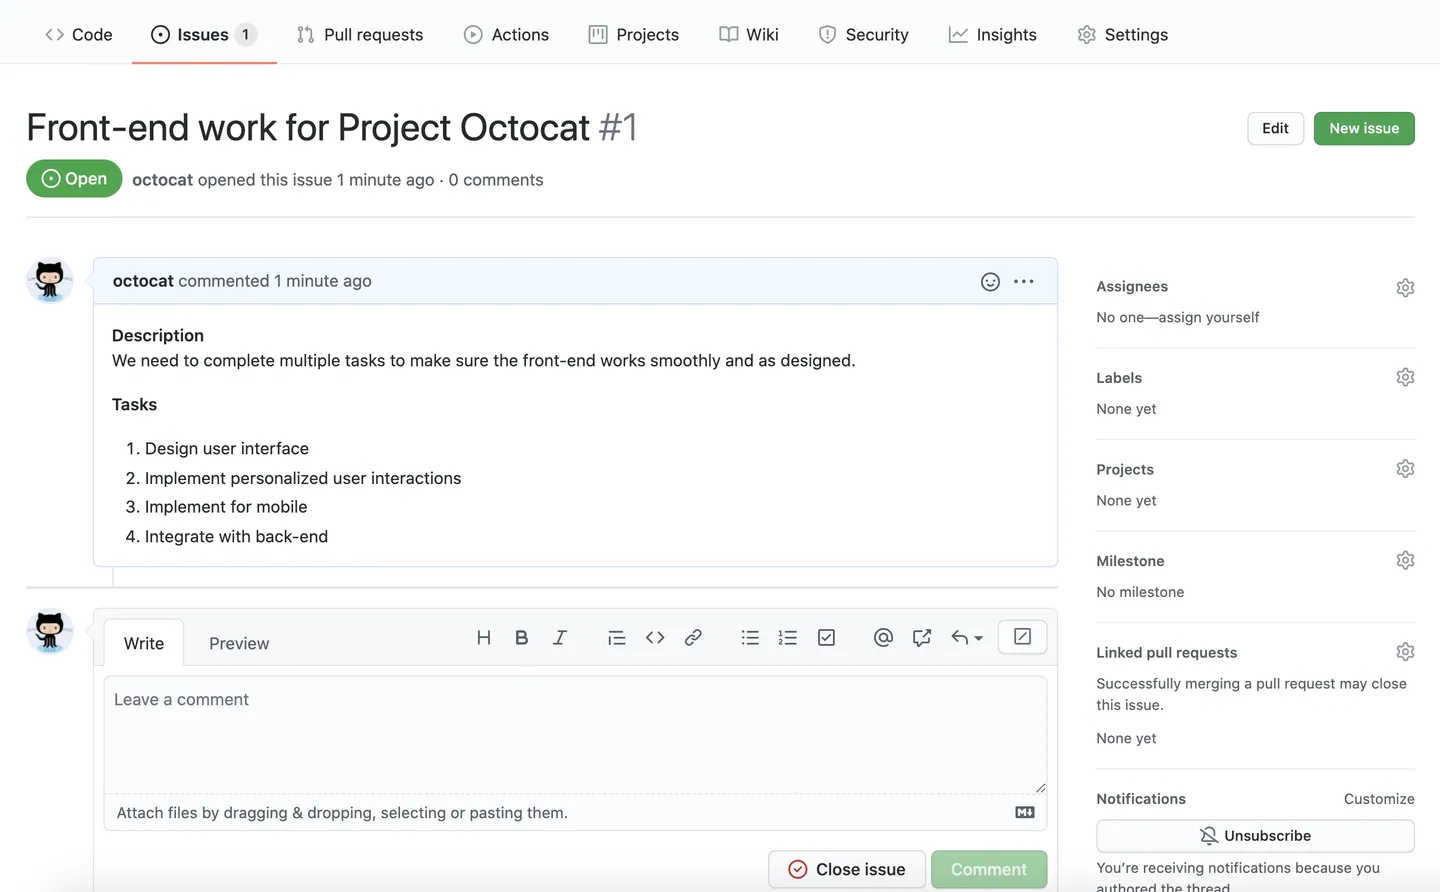
\includegraphics[width=1.00\textwidth]{images/github-issues.png}
    \caption{Captura de ejemplo de una \textit{issue} del proyecto extraída de la documentación oficial de GitHub}
    \label{fig:github-issues}
\end{figure}

GitHub Projects permite organizar el desarrollo mediante tableros Kanban que estarán poblados por cada una de las \textit{issues} del proyecto. En una vista general del tablero o \textit{board layout} (Ver \autoref{fig:github-projects-board}) se pueden distinguir las \textit{issues} por estado: si están todavía pendientes de análisis, en desarrollo, en etapa de pruebas o ya finalizada dado que ya fueron integradas a la implementación final.

\begin{figure}[htbp]
    \centering
    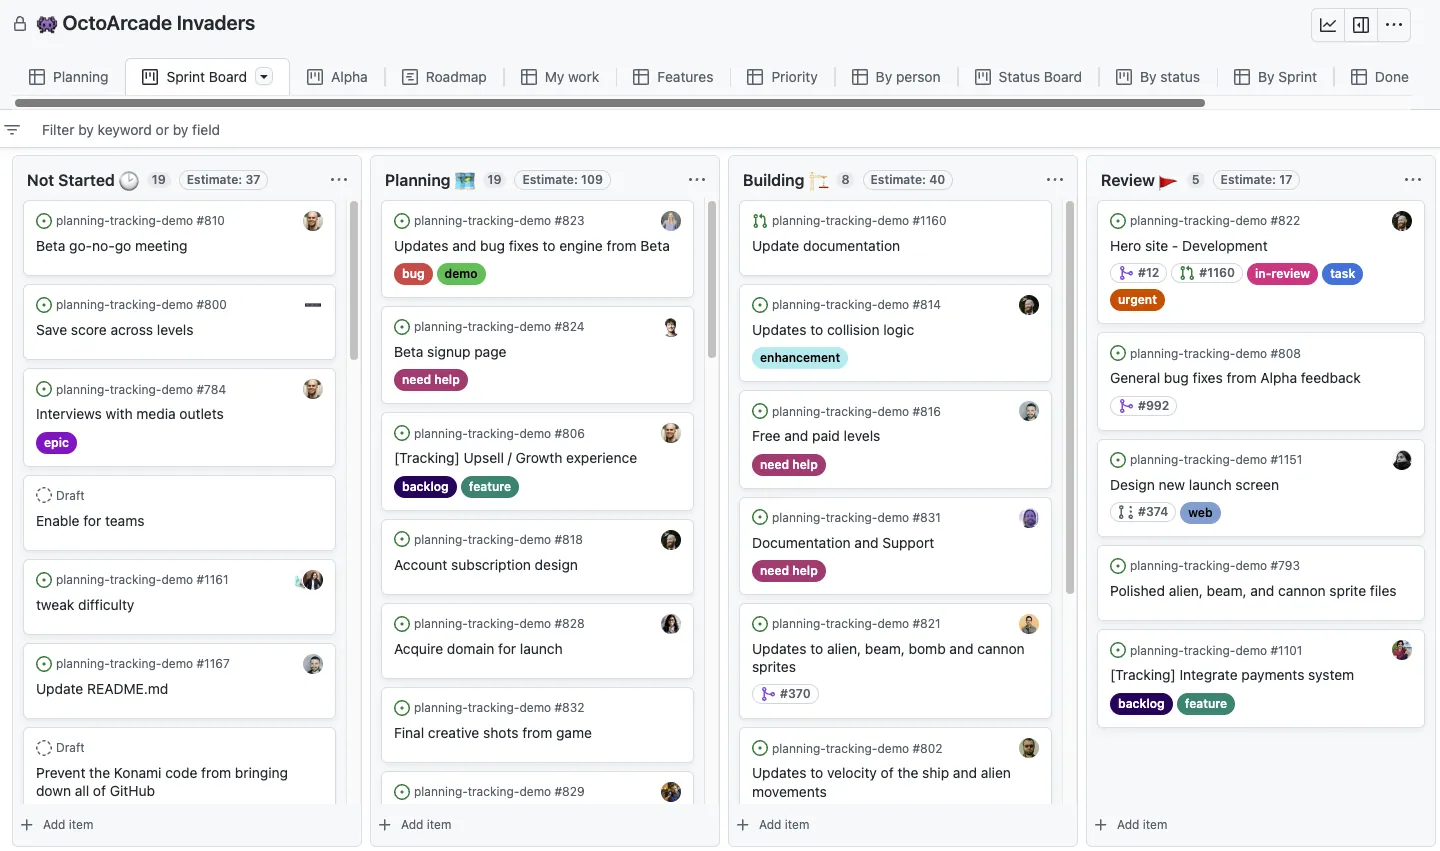
\includegraphics[width=1.00\textwidth]{images/github-projects-board.png}
    \caption{Captura de ejemplo de una vista \textit{board} del proyecto extraída de la documentación oficial de GitHub}
    \label{fig:github-projects-board}
\end{figure}

También se ofrece una vista del ciclo de vida de desarrollo o \textit{roadmap} (Ver \autoref{fig:github-projects-roadmap}) donde se puede apreciar la dimensión tiempo en cantidad de semanas y cómo las tareas se fueron resolviendo en cada momento.

\begin{figure}[htbp]
    \centering
    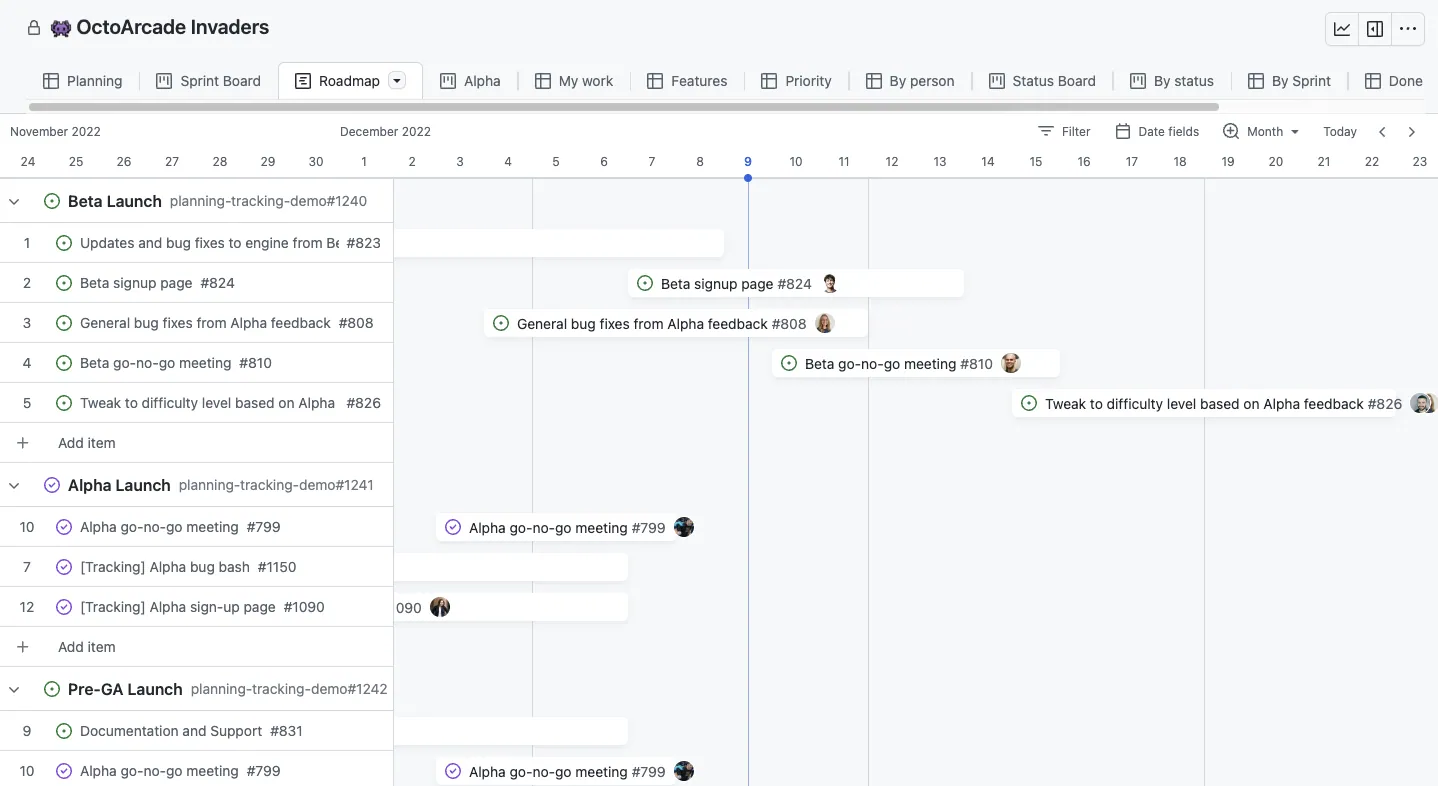
\includegraphics[width=1.00\textwidth]{images/github-projects-roadmap.png}
    \caption{Captura de ejemplo de una vista \textit{roadmap} del proyecto extraída de la documentación oficial de GitHub}
    \label{fig:github-projects-roadmap}
\end{figure}

\FloatBarrier
\section{Bibliografía}
\renewcommand{\refname}{Referencias}
%\bibliographystyle{IEEEtran}
\bibliographystyle{apacite}
\bibliography{export}

\end{document}  